\section{Tape-Out}
\label{sec:tapout}
The initial objective was to conclude the chip design phase of this project within the scope of the first project thesis. Unexpected delays in the timeline however led us to miss the initial tape-out deadline. A substantial portion of this delay stemmed from the necessity to overhaul the buck-boost converter regulator loop. The regulator loop previously implemented average current-mode control which necessitates stringent requirements for the current measurement circuit. As a result, the design was altered to implement peak current-mode control as is has more manageable requirements for the current measurement. Despite the provision of an extended timeline, finalizing the design before the deadline remained a challenging task requiring the removal of some nonessential features in oder to meet the deadline. 

\subsection{Buck-Boost Converter}
The layout of the buck-boost converter can be seen in  \autoref{fig:BBlayout} with annotations showing the rough floorplan of the circuit. Surrounding the converter are the four large switching transistors that significantly increased in size between initial planning in the previous thesis and to what was ultimately implemented. The exact values and sizes are listed in \autoref{tab:spec_pmos} and \autoref{tab:spec_nmos}. The largest contributor to the losses in the power-stage surprisingly are the metal trace resistances which increased the theoretical $R_{DS,on}$ of the \ac{PMOS} power transistors from \qty{58.3}{\milli\ohm} to an effective value of \qty{240}{\milli\ohm} in post-layout simulations. These metal resistances could not be reduced through wider traces as the maximum metal density for manufacturing was the limiting factor.\\
The large empty space above the error amplifier in \autoref{fig:BBlayout} was initially intended for a temperature sensing circuit in order to measure the rough temperature of the power electronics and to disable operation in case of an over temperature event. Due to the tight timeline, the layout of this circuit was not completed as the priority was shifted towards finishing other more critical circuits. As a result of the same issue the implementation of \ac{DFT} functionality was kept to a bare minimum and only includes the ability to measure the oscillator clock frequency, the bandgap reference voltage and the internal current reference. Consequently, the chip is with respect to troubleshooting a black-box with no possibility to measure some important internal signals.


\begin{table}[H]
    \centering
    \begin{tabular}{|c|c|c|}
        Characteristic & Planned Value & Implemented Value \\
        \hline
		 Typ. $R_{DS,on}$ & \qty{113}{\milli\ohm}  & \qty{58.3}{\milli\ohm} \\
         \# of Transistors & \qty{4834}{}  & \qty{9408}{} \\
		 Width & \qty{96.7}{\milli\meter} & \qty{188.2}{\milli\meter}\\
		 Size & \qty{1000.2}{\micro\meter} x \qty{486.8}{\micro\meter} & \qty{1228.8}{\micro\meter} x \qty{764.4}{\micro\meter}
    \end{tabular}
    \caption{Specifications of the power \ac{PMOS}}
    \label{tab:spec_pmos}
\end{table}

\clearpage
\begin{table}[H]
    \centering
    \begin{tabular}{|c|c|c|}
        Characteristic & Planned Value & Implemented Value \\
        \hline
		 Typ. $R_{DS,on}$ & \qty{72.8}{\milli\ohm} & \qty{37}{\milli\ohm} \\
         \# of Transistors & \qty{2800}{}  & \qty{6080}{} \\
		 Width & \qty{56}{\milli\meter} & \qty{121.6}{\milli\meter} \\
		 Size & \qty{641.4}{\micro\meter} x \qty{483.1}{\micro\meter} & \qty{972.8}{\micro\meter} x \qty{688}{\micro\meter}
    \end{tabular}
    \caption{Specifications of the power \ac{NMOS}}
    \label{tab:spec_nmos}
\end{table}

\begin{figure}[h]
    \centering
    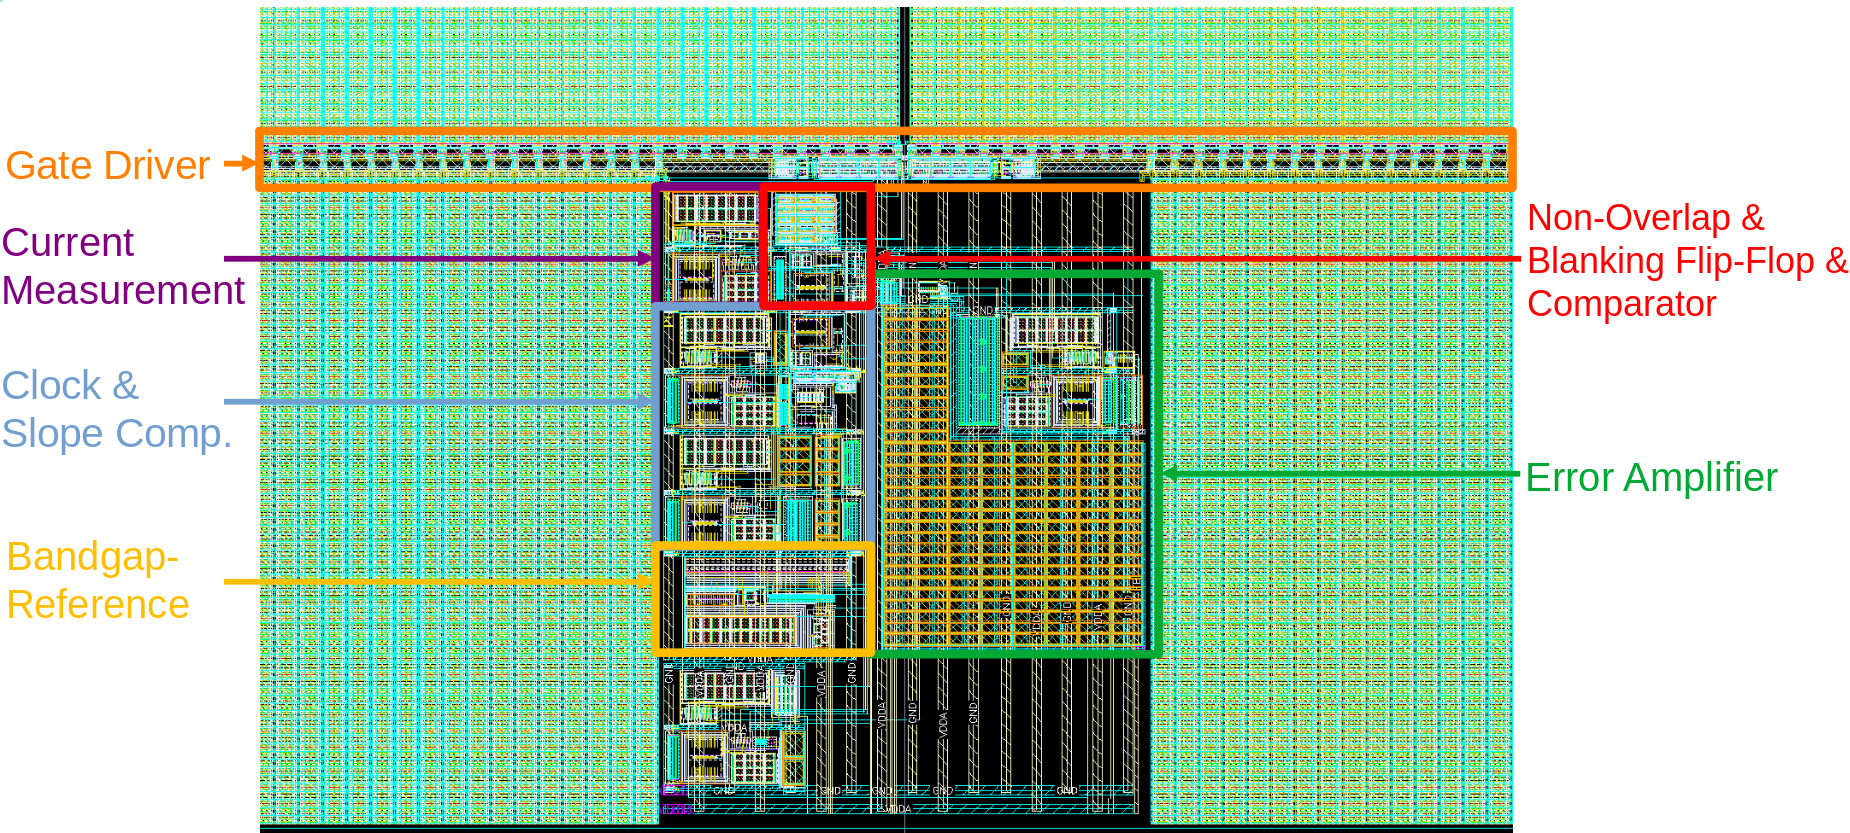
\includegraphics[width=1\textwidth]{../ASIC-DESIGN-2/images/07_DCDC/BuckBoostLayout.png}
    \caption{Layout of the buck-boost converter regulator surrounded by the large power stage transistors}
    \label{fig:BBlayout}
\end{figure}

\clearpage

\subsection{Overall Chip Floorplan}
As can be seen in \autoref{fig:chiplayout}, this design is significantly pad limited as opposed to core limited. The entire lower right corner is unused and in general the lower third is sparsely populated. Conversely the upper two thirds is almost entirely filled the the buck-boost converter circuit with the majority of the area taken up by the four large switching transistors. They were maximized in size to reduce conversions losses and even take up the majority of the entire chips area. A large number of pads were used in parallel for the converters input, output and switching nodes to meet the current handling requirements and not exceed the recommendation of \qty{50}{\milli\ampere} per pad. In the bottom left the digital circuitry for the \ac{SPI} periphery and internal registers can be seen as well as supporting circuitry like the \ac{POR} and bandgap voltage reference. 
\begin{table}[H]
    \centering
    \begin{tabular}{|c|c|}
        Property & Value \\
        \hline
        Function & Buck-Boost Converter \\
        Package & QFN48 7x\qty{7}{\milli\meter} \\
        Process & X-FAB \qty{350}{\nano\meter} \\
		Size & \qty{2712}{\micro\meter} x \qty{2952}{\micro\meter} \\
        Area & \qty{8.006}{\milli\meter\squared}
    \end{tabular}
    \caption{ASIC Properties}
    \label{tab:spec_asic}
\end{table}
\begin{figure}[h]
    \centering
    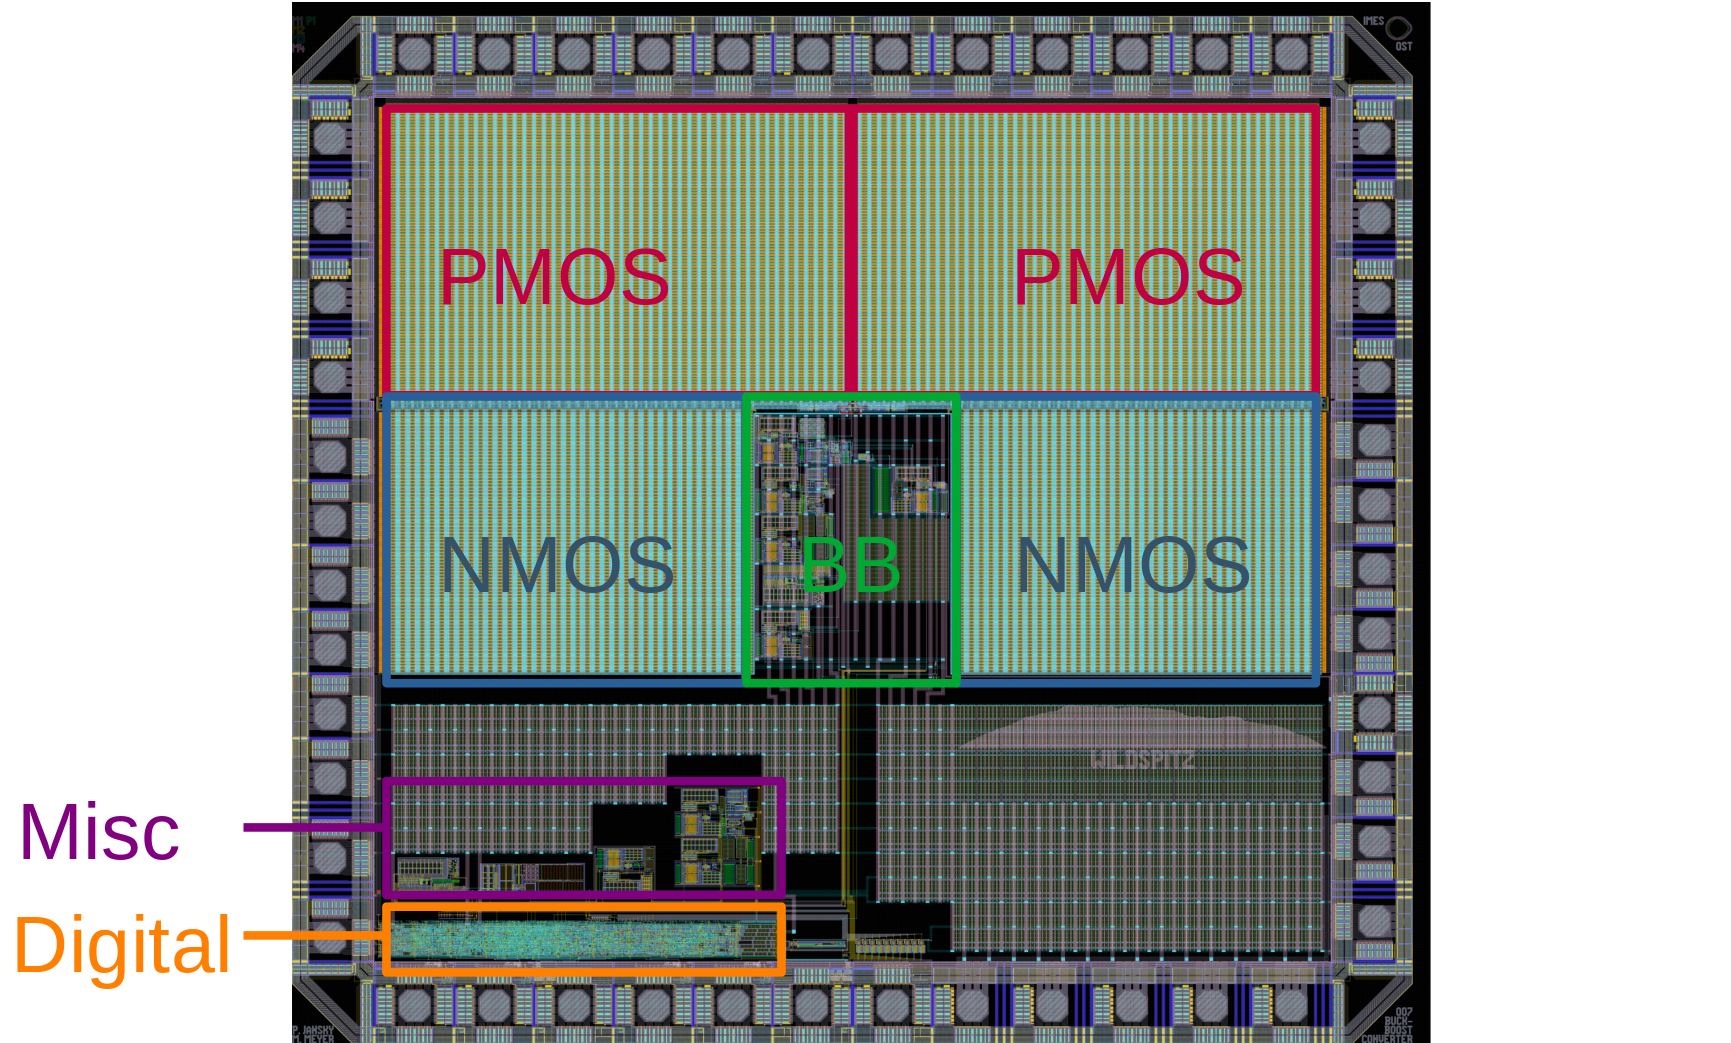
\includegraphics[width=1\textwidth]{../ASIC-DESIGN-2/images/07_DCDC/ChipLayout.png}
    \caption{Floorplan of the entire chip with annotations}
    \label{fig:chiplayout}
\end{figure}
\subsection{Package}
In \autoref{fig:package}, the QFN-48 package of the chip is illustrated with the pinout of the device marked. It is evident that there are two distinct ground connections, namely a power ground GND\_2 for the switching converter and GND as a general purpose ground for the internal circuits. The same applies to the supply voltages with V\_IN being the power input of the switching converter and VDD\_D being the internal logic supply. While these two domains are independent and not internally connected, they typically would be connected together on the \ac{PCB}. It is however advisable to separately bypass the power domains and separate them with a ferrite bead to minimize switching noise interference on the logic supply. The full pinout can be seen in \autoref{fig:package}.
\begin{itemize}
	\item \textbf{A\_OUT:} Analog test pin to mux out internal signals. See also \autoref{subsec:spi_interface}
	\item \textbf{D\_OUT:} Outputs internal clock when enabled. See also \autoref{subsec:spi_interface}
	\item \textbf{FB:} Feedback to overwrite output voltage by external voltage divider \\
            $V_{OUT} = \qty{1.25}{\volt} \cdot \frac{R_{FBT}}{R_{FBB}}$; $(R_{FBT}+R_{FBB}) \ll \qty{100}{\kilo\ohm}$
	\item \textbf{GND:} Ground of digital logic and internal circuits
	\item \textbf{GND\_2:} Ground pins for DC/DC converter
	\item \textbf{L\_IN/L\_OUT:} Connection to an external \qty{47}{\micro\henry} coil
	\item \textbf{RST:} Active high reset, resets the whole chip including the internal registers
	\item \textbf{SPI*:} SPI interface connections
	\item \textbf{VDD\_D:} Supply of digital logic and internal circuits
	\item \textbf{V\_IN:} Supply voltage for power stage
	\item \textbf{V\_OUT:} Buck-boost converter output, nominally \qty{5.0}{\volt}
\end{itemize}
\begin{figure}[h]
	\centering
	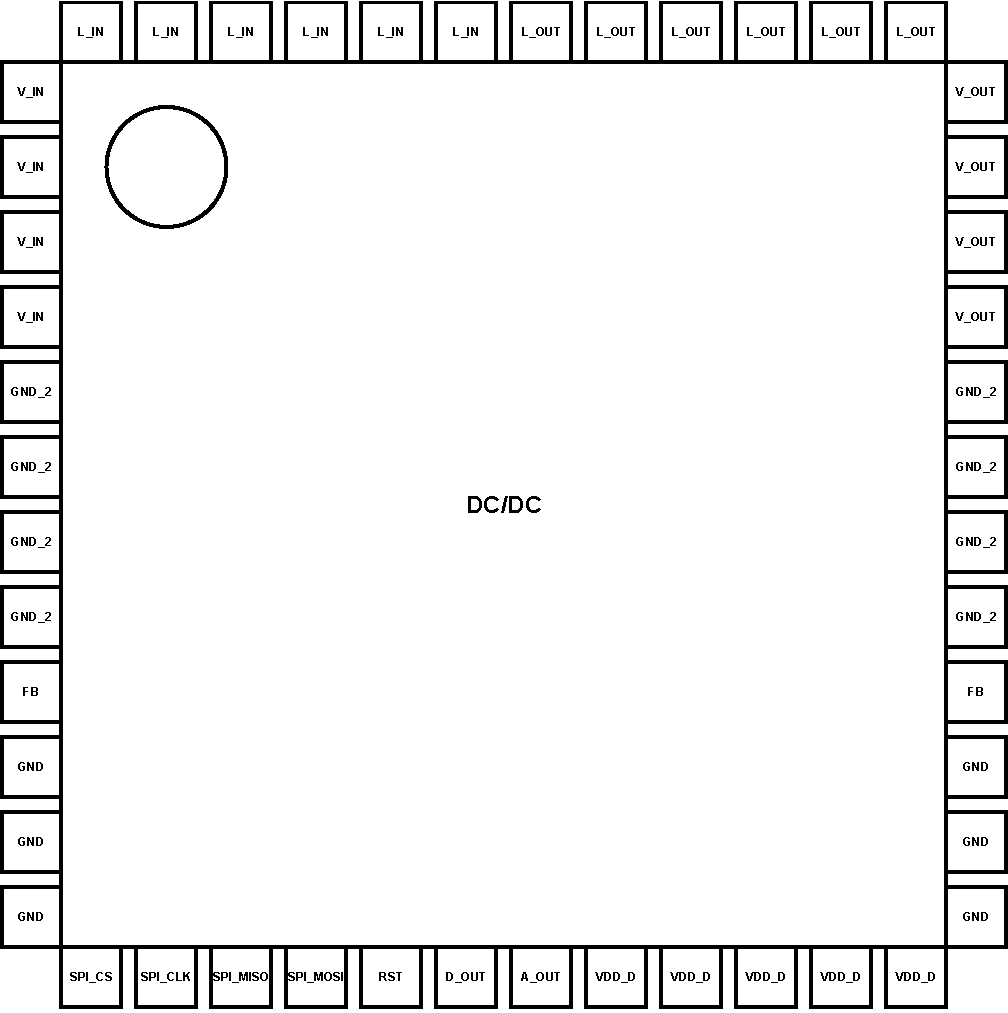
\includegraphics[width=1\textwidth]{../ASIC-DESIGN-2/images/pakage.pdf}
	\caption{QFN-48 Device Pinout, Top View}
	\label{fig:package}
\end{figure}
